\documentclass[runningheads]{llncs}
\usepackage{graphicx}\usepackage{placeins}
\usepackage{fancyvrb}
\usepackage[bf]{caption2}
\usepackage{amssymb,amsmath}
\usepackage{comment}
\begin{document}
\pagestyle{headings}
\mainmatter

\title{Using Genetic Algorithms to Generate Test Suites}
%Each page title
\titlerunning{}
%Authors
\author{Austin Barket \and Randall Hudson}
%Authors on each page
\authorrunning{Austin Barket and Randall Hudson}
%University Address and contact information
\institute{Department of Computer Science\\
The Pennsylvania State University at Harrisburg\\
Middletown, PA 17057\\
\email{amb6470@psu.edu, rvh5220@psu.edu} } \maketitle
%Document text starts here ...

\begin{abstract}
This paper applies techniques of genetic algorithms to the problem of finding test suites that cover every edge or predicate in a programs control flow graph. It differs in other applications of genetic algorithms to software testing in that the organisms are test suites rather than test cases. Experimental results show....
\end{abstract}


\section{TODO}

\begin{itemize}
\item Make nomenclature consistent, so if its called Medium-One somewhere and Medium-Hard somewhere else we need to pick one
     \begin{itemize}
     \item For the medium whatever graphs, I was thinking the name HardLeft and HardRight would be better names, thoughts?
     \end{itemize}
\item Add any missing citations
\item Finish the abstract
\item Experimental results section
     \begin{itemize}
     \item I think this is pretty much done. Not sure if the parameter test should be in the tables
	     or just discussed in a more theoretical context.
	     \begin{itemize}
          \item I think its fine to just discuss it afterwards.
         \end{itemize}
     \end{itemize}
\item Discussion Section
     \begin{itemize}
     \item Figure out what to say
     \end{itemize}
\item Conclusion Section
     \begin{itemize}
     \item Concluding remarks
     \item Future work
     \end{itemize}
\item Read over the copy and pasted sections from proposal to make sure it all makes sense in this new context.
\item General: find any thing that needs reworded, pruned, etc and fix.
\end{itemize}

\section{Introduction}
Software testing is a tedious and expensive process, costing as much as 50\% of a projects budget \cite{meyers1}. One reason for this is the fact that the input domain for programs tends to be extremely large, often times infinite; this makes it impossible to test all possible inputs for a program \cite{meyers1}. Thus, testers spend a large portion of their time simply searching/designing good tests. One aspect of automatic testing research aims to alleviate this burden via the automatic generation of tests.

Automatic test generation can be characterized by the creation of some system that when fed information about a program will attempt to generate good tests for that program. In model based testing, one such method for automatic test generation, engineers must design a model of the system using the functional requirements for the system; the model then generates tests cases to test the functional requirements \cite{model2}. In rule based test generation, testers design a framework of rules, generally built around predicate statements; this framework then dictates the creations of test cases based on the predicate statements in the code \cite{chang3}. These are two of the common methods used in automatic test generation. These methods generally require some upfront design costs before use. 

Genetic algorithms represent a third, and perhaps more interesting, method of automatic test generation. Tests, or test suites, take the role of the organisms in this genetic algorithm while their coverage, e.g. branch, conditional, etc, determines their fitness \cite{sthammer4}. This method represented an underexploited area of research and will be further examined in this paper. 

\newpage
\section{Problem Definition}
In high-level terms the problem succinctly presents itself as such: automatically generate good tests for a given program; but this leaves several open questions, such as ``what information if any can be gotten from the program to help design the tests?'' and ``what constitutes a good test?'' The field of structural testing will help answer both of these questions.

In any given program there are multiple paths in which flow of control can traverse; these can be represented by a control flow graph (CFG); predicates, i.e. conditional statements in the code, determine which path to take [1]. Structural testing encompasses the use of such information to design tests [1].

When evaluating a test's coverage, the predicates, and the flow of control they affect, play an important role. Consider the following simple metric: A test suite should cover every possible path in a program at least once. Using the control flow graph one can easily evaluate the quality of tests against this metric. A good test suite then becomes one in which most if not all of the possible paths are taken at least once. Structural testing uses this metric, and similar metrics, as its primary evaluation method for tests.

The problem to solve can now be stated with more detail: automatically create a test suite that covers all, or most, paths in a programs control flow graph. It is the authors' intention to solve this problem with a genetic algorithm. 

To design a genetic algorithm that solves this problem it will need the following information: the input parameters for the program, the control flow graph, and the predicates affecting each path. The output would consist of a population of test cases or test suites, depending on design decisions, that should consist of good tests. 

\newpage
\section{Related Work}
Using genetic algorithms to generate tests represents a relatively new area of research, with the first published results dating from only 1992 \cite{apps5}. Initially, genetic algorithms evolved tests that would ensure all predicates for a single path of execution were true\cite{limits6}. Later, Watkins created an adaptive fitness function that would create tests for one particular branch of the control flow graph and then switch to a different branch once some tests were found; this approach allowed a single run of the genetic algorithm to attempt to evolve the tests needed for full branch coverage\cite{limits6}. Watson's results showed that a genetic algorithm, compared to random testing, required ``an order of magnitude fewer tests to achieve path coverage…''\cite{limits6} 

Up to this point, the fitness functions viewed a branch's predicate as just a boolean function, that is true or false; this did not take full advantage of white box testing in which the exact details of each predicate can be known. Sthammer wished to use information about these predicates to create boundary value tests. He accomplished this by using a distance function that reported the distance between a test's current values for a predicate and what values that predicate needed to be true. Sthammer's showed that his technique preformed better then a random search. 

Pargas et al proposed the used of a control-dependence graph instead of a control flow graph to guide the search of test cases. They implemented this technique in a parallelizable algorithm called GenerateData\cite{pargas8}. When tested on programs with control flow graphs of cyclomatic complexity of seven significant improvements over random search were reported\cite{pargas8}.

The newest genetic algorithms attempt to make use of past information in some way. In Beuno and Jino's research they used information about past runs of the genetic algorithm to influence the creation of the initial population used in a new run\cite{limits6}. ``The results with their six small test programs were promising.''\cite{limits6} Berndt et al try to take advantage of past information in a different way. Their algorithm includes a ``fossil record that records past organisms, allowing any current fitness calculations to be influence by past generation.''\cite{limits6}

More recent work has been done by Gordon Fraser, Andrea Arcui, and others in their development of the evolutionary test suite generator EvoSuite \cite{FraserTestSuites}. This is some of the earliest research using test suites instead of test cases for the organism's chromosome. Test cases are also unique in that they are composed of Java statements rather than the program's input parameters. Both test cases and test suites can change size during the simulation. EvoSuite has proven to be a powerful method for automatic test generation \cite{Fraser}.






\newpage
\section{Our Work}
Our approach focused on the idea of using test suites as an organism's chromosome rather than test cases. We also added some new evolutionary algorithm techniques that did not appear to be widely used in other literature for this problem. Additionally, we implemented several test programs of varying difficulty. Each of these items will now be discussed in turn.

As noted above, test suites compose the population and each of these consists of multiple test cases. The number of test cases for a given test suite was decided to be the sum of the number of edges and predicates in the target control flow graph; this would ensure every test suite would be able to cover all possible branches and predicates in the target program. Each test case contains an array of values that represent input parameters to the program being tested. For the purposes of this research, input parameters were restricted to the domain of 32-bit integers.

Since an organism’s chromosome is now an entire test suite, one may think the simulation should try to evolve organisms with the maximum possible coverage, but this is not the case. Even if no single organism has full coverage, if the population as a whole covers everything, then there is no need to continue the simulation. In order to still get a single test suite with full coverage, as the simulation discovers test cases that offer new coverage, it records their inputs. 

Many of the GA’s from the literature for this problem are rather simplistic \textbf{TODO: add citations}. To improve upon them we implemented and tested many techniques, including several types of fitness scaling, several base fitness functions, several mutation operators for test suites, tournament selection, several types of local optimizations, several adaptive parameters et al… Most of these were not fit enough to survive our culling. The subset that did survive includes local optimization for test cases, fitness sharing, and adaptive ranges. These are discussed in more detail in the algorithm sub-section.

Test programs are provided to the algorithm in the form of executable CFGs. A CFG represents linear blocks of instructions from the target program as nodes. The edges represent possible different directions the flow of control can follow when it reaches a predicate.  When implementing multiple condition coverage, one could simply expand each predicate, turning it into one predicate for each possible outcome; this has its advantages but can make tracking branch versus MCC coverage harder. Our implementation uses edges solely for possible directions of control in the original target program. A separate set for predicates is kept, and each node (aka block) is responsible for tracking its predicates. This means that in our implementation, covering all edges equates to achieving 100\% branch coverage and covering all predicates equates to achieving 100\% multiple condition coverage. 

\subsection{Algorithm}\label{sec:Alg}
At a high level the algorithm is based around a simple observation from the field of software testing. Programs, although having very large input domains, typically only have a few equivalence classes of their parameters. Here an equivalence class refers to a range of values for a parameter such that when input to the program cause the same flow of control. e.g. A program with one input and the simple predicate $ x < 0$, has two equivalence classes for the value of x [int\_min, -1] and [0, int\_max]. As a result this program only needs two test cases for achieve full coverage.

Of course, unlike the problem above, most meaningful programs have several parameters and typically have complex relationships between input parameters that drive the control flow of the program. The algorithm proposed here finds much of its basis in a simplifying assumption of these complex relationships. Consider a program with three inputs x, y, and z. Let R1, R2, and R3 be ranges in the domains of these inputs. Suppose this program requires a test case of the following form to cover a specific path in the CFG $\{ x \in R1, y \in R2, z \in R3 \}$. The assumption made is that $\{ x \in R1, y \in R1, z \in R1 \}$, $\{ x \in R2, y \in R2, z \in R2 \}$, and $\{ x \in R3, y \in R3, z \in R3 \}$ will each cover different paths in the control flow graph. 

The algorithm attempts to find a set of promising ranges using this assumption. Then applies a genetic algorithm to search the space of test cases resulting from various combinations of parameters from these ranges. Of course this is not perfect and it would not be difficult to construct a program that violates this assumption. However our results show that this method can be effective in finding the vast majority of coverage in test programs with a range of complexity.

The following section has been broken down into the subsections for each major aspect of the proposed algorithm. First, the main simulation loop is provided to give context throughout the rest of the sections. The notion of input parameter ranges and the simulation's range set is then introduced, followed by a discussion of the population initialization. Fitness calculation and association with organisms is explored; then the tools used for test case generation, including test case crossover and mutation, test suite crossover and mutation, local optimization and range set adaptation are studied.

\begin{comment}
Do you think this name is ok? I ask because techincally it shows both the initialization and the main loop. 
We could call it somthing like 'Algorithm Overview' or 'Simulation Algorithm'.
\end{comment}
\subsubsection{Main Simulation Loop}

%============================= Main Loop Alg =====================
\begin{figure}[h!]
	\begin{center}
		\hrule
		\medskip
\begin{Verbatim}[fontfamily=tt, xleftmargin=10pt, commandchars=\\\{\},
codes={\catcode`$=3\catcode`^=7\catcode`_=8}]
   $currentGen\leftarrow0 $
   
   FindGoodRanges()
   BuildPopulation()
   
   do \{
      UpdatePopulationsFitness()
   
      Proportionally select a test suite, $ts$, from the population
      Use $ts$ for test case crossover and mutation to get $tc$
      If $tc$ is not null add it to $ts$ by replacing a duplicate test case
   
      if $currentGen$ is multiple of 10
         TryLocalOptimization()
   
     if no improvement for $\ge20$ generations and $currentGen$ is multiple of 100
        AdaptRanges()
   
     if no improvement for $\ge20$ generations and $currentGen$ is multiple of 30 
        Proportionally select two test suites from the population
        Do crossover and mutation on these to get children
        Replace both parents with the children
     fi
   
     $currentGen \leftarrow currentGen+1$
   \} while ending criteria has not been met
\end{Verbatim}
\hrule
	\end{center}
	\caption{Algorithm for main simulation loop \label{fig:simLoopAlt}}
\end{figure}
\FloatBarrier
%============================= End Main Loop Alg =====================

\subsubsection{Initializing the Range Set}

The algorithm maintains a set of promising input parameter ranges throughout the simulation. Any time a new test case needs to be generated the simulation can query this range set for good ranges; the simulation can then pick parameters from those ranges for the new test case. 

A range includes a start value and an end value, as well as an array of input parameter buckets. The buckets are partitions of size 25 within the range, e.g. the range [0, 74] would contain the following array of buckets [ [0, 24], [25, 49], [50, 74] ]. These buckets contain counts of how many times that sub-range was used to provide some unique coverage for the population. Summing the counts in these buckets gives the usefulness for that range.

At the start of the simulation the FindGoodRanges() procedure is run to find promising ranges of input values and add them to the global range set. This procedure loops, starting with a range around zero and extending in both directions towards max and min integer, generating a single test case from each range. If a test case provides coverage that has not yet been seen during this initial procedure, its corresponding range is added to the global range set. 

This procedure can be repeated using various range sizes, which in some cases enabled the algorithm to find additional coverage and ranges not found in previous iterations. However, this is an expensive procedure; thus, only two iterations were used, first with a range of size 5000, then with a range of size 2500. This provided a good set of initial seed ranges for the genetic algorithm to utilize, while not taking too long to complete.


%============================= Range Search Alg =====================
\begin{figure}[h!]
\begin{center}
\hrule
\medskip
\begin{Verbatim}[fontfamily=tt, xleftmargin=10pt, commandchars=\\\{\},
codes={\catcode`$=3\catcode`^=7\catcode`_=8}]
$\hbox{FindGoodRanges}()$  
   $rangeSet \leftarrow$ Empty Range Set
		
   for ( $size \in \{5000, 2500\}$ ) 
      $posStart \leftarrow -size/2$
      $negStart \leftarrow size/2$
		
      while $posStart + size < max\_int$ and $negStart - size > min\_int$ \{
         $posRange \leftarrow$ [posStart, posStart + size]
         $negRange \leftarrow$ [negStart, negStart - size]
		
         $posTC \leftarrow$ test case in posRange
         $negTC \leftarrow$ test case in negRange
		
         if (posTC covers anything new)
            add posRange to rangeSet
		
         if (negTC covers anything new)
            add negRange to rangeSet
		
         $posStart \leftarrow posStart + size$
         $negStart \leftarrow negStart - size$
      \}
   end-for
		
   return $rangeSet$
\end{Verbatim}
\hrule
\end{center}
\caption{Algorithm for finding good ranges \label{fig:ranges}}
\end{figure}
\FloatBarrier
%============================= End Range Search Alg =================

\subsubsection{Initializing the Population}

During initialization each organism in the population uses only a single range from the simulation's range set to generate all its test cases. In this way the algorithm starts by searching the space of test cases possible using only parameters from a single range. The genetic operators defined below then attempt to search the possible combinations of these ranges, focusing on the ranges and organisms that have been most fruitful in generating unique coverage thus far.

\subsubsection{Fitness}

\paragraph{Coverage Metadata}
The algorithm maintains three levels of coverage metadata for the purposes of fitness calculation. First, each test case is assigned coverage by running it against the CFG. Each test suite then maintains counts of the number of times its constituent test cases covered each edge and predicate. Finally, the population maintains sums of the coverage counts across all of the test suites.

\paragraph{Fitness Sharing}
The algorithm assigns fitness for an organism based off both its coverage and the population's coverage; this is a form of fitness sharing. Each edge or predicate has a base score associated with it. The score for a particular edge or predicate is split amongst all the test suites that cover it. The motivation for using fitness sharing is the following: if many organisms cover a particular edge, then it must be easy to reach and thus organisms should receive less fitness for covering it; however, if only one organism in the population covers an edge, then that organism should receive a higher fitness. 

\subsubsection{Crossover, Mutation, and Replacement}

Test suites and test cases each have their own crossover operator. Both operators use normal k-point crossover and fitness proportional selection. However, the test case operator only selects one test suite and then selects test cases at random from that test suite to crossover. The simulation attempts test case crossover several times before giving up; this is to increase the chance of finding good parameter combinations, assuming the range search has narrowed in on good ranges.

Mutation and replacement immediately follow both forms of crossover. The simulation uses point mutations in both cases, each with probability $P_m$. For test suites, mutation involves creating a new test cases out of the most useful ranges in the range set. After test suite crossover, the algorithm always replaces both parents. For test cases, mutation involves changing a parameter to a new value selected using a normal distribution around the parameter's original value. Child test cases only find their way into the parent test suite if they offer new coverage. 

Even though these two operators are similar they each serve a different purpose. Test suite crossover causes a greater change in the partaking organisms by swapping a significant number of entire test cases between the parents. Since, each test case was created with certain ranges, this also has the effect of mixing up the ranges in a test suite. Since this is a disruptive operation, the algorithm performs test suite crossover only after several generations of no improvement in coverage. Test case crossover, on the other hand, makes much smaller changes to a test suite, by mixing up the parameters between two test cases. Thus the ranges of parameters available within the organism do not change, but the coverage of the suite may improve as a result. This was designed to be the main genetic operator for test case search, and thus is run every generation. The hope is that test suite crossover will help the suite get the needed ranges and then test case crossover will be able to combine those ranges into more useful test cases.

%============================= Test Case Cross Alg =====================
\begin{figure}[h!]
	\begin{center}
		\hrule
		\medskip
		\begin{Verbatim}[fontfamily=tt, xleftmargin=10pt, commandchars=\\\{\},
		codes={\catcode`$=3\catcode`^=7\catcode`_=8}]
$\hbox{TestCaseCrossover}(cutPts, P_m)$  
   Proportionally select a test suite, $ts$, from the population

   for $i=0$ to $100$
      From$ ts $ select two random test cases,$ tc1 $and$ tc2 $

      $child1, child2 \leftarrow $crossover($tc1$, $tc2$, $cutPts$)
      $child1.$mutate($P_m$)
      $child2.$mutate($P_m$)

      if $child1$ is covering anything not covered by ts
         $ts$.addTestCase($child1$)
         break
      else if $child2$ is covering anything not covered by ts
         $ts$.addTestCase($child2$)
         break
   end-for
		\end{Verbatim}
		\hrule
	\end{center}
	\caption{Algorithm for test case crossover \label{fig:tcCross}}
\end{figure}

\FloatBarrier
\subsubsection{Local Optimization}

Two simple local optimization techniques are used, but the structure of both is very similar. The LocalOptFromParameters function will take a test case and, beginning with a small neighborhood size, will begin looking at other test cases in the neighborhood of that test case. The LocalOptFromZero function tries to pull the test case's parameters closer to zero. This was added because values in the neighborhood of zero, such as 1, -1, or 0, can drastically alter the flow of the program being tested, but because the search space was so large, the simulation was unable to find these values without help. Both functions explore each neighborhood several times, then expand the neighborhood to try again if no new coverage could be found. The TryLocalOptimization procedure called from the main simulation loop chooses, with equal probability, one of these heuristics to apply. If at any point during either procedure a test case is found that offers new coverage to the simulation, it is added to the organism by replacing a duplicate test case.

%============================= Local Opt Alg =====================
\begin{figure}[h!]
	\begin{center}
		\hrule
		\medskip
		\begin{Verbatim}[fontfamily=tt, xleftmargin=10pt, commandchars=\\\{\},
		codes={\catcode`$=3\catcode`^=7\catcode`_=8}]
$\hbox{LocalOptFromParameters}(testCase)$
   $neighborhoodSize\leftarrow5 $
   for $i=1$ to $500$ 
      $temp\leftarrow$$testCase$
      for $j=1$ to $150$
         for each parameter, $p$ in temp
            set p to a random value in the neighborhood of p
         end-for     
         if $temp$ covers anything not covered in the population return$ temp $
      end-for
      $neighborhoodSize\leftarrow$$neighborhoodSize+5$
   end-for

   if no improvement was ever found then return null
		\end{Verbatim}
		\hrule
	\end{center}
	\caption{Algorithm for local optimization from existing parameters \label{fig:lcOptFP}}
\end{figure}
\begin{figure}[h!]
\begin{center}
\hrule
\medskip
\begin{Verbatim}[fontfamily=tt, xleftmargin=10pt, commandchars=\\\{\},
codes={\catcode`$=3\catcode`^=7\catcode`_=8}]
$\hbox{LocalOptFromZero}(testCase)$
   $neighborhoodSize\leftarrow5 $
   for $i=1$ to $1000$ 
      $temp\leftarrow$$testCase$
      for $j=1$ to $150$
         for each parameter, $p$ in temp
            95\% of the time set $p$ to a random value in the neighbor of zero
            5\% of the time set $p$ to $p/2$
         end-for     
         if $temp$ covers anything not covered in the population return$ temp $
      end-for
      $neighborhoodSize\leftarrow$$neighborhoodSize+5$
   end-for
		
   if no improvement was ever found then return null
\end{Verbatim}
\hrule
\end{center}
\caption{Algorithm for local optimization around zero \label{fig:lcOptFZ}}
\end{figure}
\FloatBarrier
%============================= End Local Opt Alg =====================


\subsubsection{Range Set Adaptation} The initial search for good ranges will probably fail to find all useful ranges; it may also think some ranges are useful which actually are not. Range adaptation aims to give the simulation the ability to remove non-useful ranges, as well as focus in on the most fruitful ranges, and find new ones that may have been missed. This procedure is only run after many generations of no improvement using the other operators.

First, the range set deletes any ranges below one standard deviation usefulness. All ranges above one standard deviation usefulness are split into two equal sized ranges, with the input parameter buckets copied accordingly to the new ranges. The two ranges immediately above and below the original range are also added to the range set. These new adjacent ranges have the same size as the original range and their usefulness values are set to half that of the original range in order to prevent them being completely ignored. Finally, the range set adds a new random range into its pool to avoid missing ranges not found during initialization or a previous range adaptation.

%============================= Adapt Ranges Alg =====================
\begin{figure}[h!]
\begin{center}
\hrule
\medskip
\begin{Verbatim}[fontfamily=tt, xleftmargin=10pt, commandchars=\\\{\},
   codes={\catcode`$=3\catcode`^=7\catcode`_=8}]
$\hbox{AdaptRanges}()$    
   for each range in rangeSet
      if ($range.usefulness < \mu-\sigma$)
         remove $range$ from the range set
      
      if ($range.usefulness > \mu+\sigma$)
         addAdjacentRanges($range$)
         splitRangeIntoTwo($range$)  
   end-for
   
   add new random range to the RangeSet
\end{Verbatim}
\hrule
\end{center}
\caption{Algorithm for adapting ranges \label{fig:adptRang}}
\end{figure}
\FloatBarrier
%============================= End Adapt Ranges Alg =====================

\subsubsection{Stopping Criteria}
The algorithm has three potential stopping criteria. 
\begin{enumerate}
	\item Achieving 100\% branch and multiple condition coverage. 
	\item 500 generations without any improvement of branch or multiple condition coverage
	\item 10000 generations have passed.
\end{enumerate}

\begin{comment}
Maybe this should be called Summary or 'Algorithm Summary' so the reader doesnt think its the actual conclusion
\end{comment}
\subsubsection{Conclusion}
The proposed genetic algorithm seeks to generate a test suite with maximal coverage by utilizing a simplifying assumption of the relationships between input parameters. First, the algorithm finds a set of promising ranges that give unique coverage when used as the sole source of parameter values. Then a genetic algorithm, with the help of local optimization and range set adaptation, searches the space of possible test cases stemming from the most promising combinations of these ranges to build a test suite with maximal branch and multiple condition coverage. The results of our tests are promising, however further inspection uncovered that the majority of the test cases that made it into the final test suite originated from the initial population and local optimization, and the genetic search did not work as well as we hoped. 


\newpage

\section{Experimental Results}

The algorithm was tested against 5 control flow graphs of varying complexity, these include a simple too high or too low number guessing program, the well known triangle problem, and three larger custom built CFGs. Our testing consisted of two steps. First, we analyzed the effect of varying the parameters of population size, mutation probability, and number of cut points on some of the implemented graphs. Based on the results of these initial tests we set up a number of final tests to perform. These will be described in detail below. 
  
\subsection{Test Programs}

\subsubsection{HiLo CFG}
This graph models a very simple program with three integer input; num1, num2, and guess. An internal variable target is computed as the product between num1 and num2. The guess parameter is compared to the target to determining if the user's guess was correct, too high, too low, not even trying (less than both num1 and num2), or equal to 0. The resulting CFG has 10 blocks, 14 edges, and 14 predicates.

\subsubsection{Triangle CFG}
The triangle problem is a very common introductory problem in the field of software testing. The program takes three inputs, each representing the length of a side of a triangle. The program then compares the sides to each other using a number of predicates to determine if the sides form an equilateral, isosceles, scalene, or violate the triangle inequality. The resulting CFG has 13 blocks, 12 edges, and 21 predicates.

\subsubsection{Hard CFG}
In an attempt to give the algorithm a more formidable test, this graph was custom designed. The idea was to have some more complex relationships between the parameters dictate the shifts in control flow. Thus in addition to conditional statements involving the traditional comparison operators between parameters, this graph utilizes the mean, standard deviation, and the sum of the parameters in its predicates. This graph takes the form of a perfect binary tree and is generally symmetric in nature as far as the types of predicates in corresponding blocks of the left and right subtrees. The hard CFG has 10 parameters, 31 blocks, 78 edges, and 150 predicates.

\subsubsection{Med Hard 1 and Med Hard 2 CFGs}
Initial testing seemed to show that Hard CFG was a little too challenging for the algorithm. In addition it exceeded the scope of the problems algorithms such as these are typically evaluated against. Thus the Hard CFG was split at the root into two subtrees, which became Mad Hard 1 and Med Hard 2. The number of parameters was pruned down to 4, naturally each subtree has 39 edges, and due to how the cut was performed Med Hard one has 74 predicates while Med Hard 2 has 79 predicates.

\subsection{Parameter Tuning} 
In hopes of finding an optimal combination of parameters for the GA, systematic tests were run on all the graphs just discussed. The details of these tests can be seen in Appendix A.

The results on all graphs showed that none of the parameters made a substantial impact on the ability of the algorithm to find coverage. Coverage ratios were generally constant across the board for each graph, regardless of what parameters were used. The only exception being that if the population size was less than the number of ranges found in the initial range search, coverage suffered by as much as 10\%. For HiLo and Triangle the algorithm maxed out coverage in less than 100 generations. For the med hard graphs the number of generations varied by no more than 400 generations, and in a mostly random manner making it hard to claim any particular combination of parameters was better than another. This seemed to indicate that the initial range search, population generation, and local optimization functions account for the majority of the coverage obtained by the algorithm.

\subsection{Results}
\paragraph{Setup}Since no particular set of parameters seemed to prevail over others, we chose to run our final tests somewhat arbitrarily with a population size of 25, 0.5 mutation probability, and 2 cut points. In order to further investigate the efficacy of the various operators, four categories of final tests were performed on each of the CFGs. First, we evaluated each CFG against the entire algorithm as described in section \ref{sec:Alg}. Then, to determine the effectiveness of the local optimization alone, we cut out all calls to test case and test suite crossover and mutation. To determine the extent the genetic operators are capable of finding good test cases, we evaluated each CFG against the algorithm without any calls to either local optimization heuristics. Finally, each CFG was run against a completely random search for comparison. The random search was given the same amount of time as the average time taken by a run of the entire algorithm on each graph. Each test was repeated 50 times and the results shown in the following tables represent the averages obtained. 


\paragraph{Description of Tables} Table \ref{tab:CovAll} reports the average branch and multiple condition coverage achieved by running the entire algorithm. Table \ref{tab:ContrAll} reports the average size, in number of test cases, of the test suites that resulted from the runs in table \ref{tab:CovAll}. In addition, Table \ref{tab:ContrAll} reports the percentage of the test cases in the final suite that came from each of the algorithm's five test case sources. Recall, test cases present in the initial population have all of their parameters sourced from a single range found during the FindGoodRanges procedure. Tests resulting from test suite mutation are built by mixing parameters from the most useful ranges in the range set, which are sampled with replacement from the range set using a usefulness proportional selection scheme. The last three columns refer to test cases resulting from the TestCaseCrossover, LocalOptFromParameters, and LocalOptFromZero procedures respectively. Tables \ref{tab:CovNoGA} and \ref{tab:CovNoLO} have the structure as table \ref{tab:CovAll} while tables \ref{tab:ContribNoGA} and \ref{tab:ContribNoLO} have the same structure as table \ref{tab:ContrAll}, but correspond to the two partial forms of the algorithm mentioned in the Setup paragraph above. These allow for more thorough analysis of the roles played by each major operator in the algorithm, and enable us to draw some better conclusions about their search power.

\begin{table}[h!]
	% Entire Algorithm	- 	Coverages
	% Number of tests per point: 50 *)
	% Maximum Generations: 10000 *)
	% {Population Size: 25, Cut Points: 2, Mutation Prob: 0.5} 
	\begin{center}
		\begin{tabular}{| l | c | c | c | c |}
			\hline
			CFG             & Branch Coverage & MCC Coverage & Generations & Run Time \\ \hline
			HiLo            & 100\%           & 100\%        & 46          & 1s       \\ \hline
			Triangle        & 100\%           & 95\%         & 521         & 6s       \\ \hline
			Medium-Hard-One & 92\%            & 87\%         & 1027        & 26s      \\ \hline
			Medium-Hard-Two & 92\%            & 90\%         & 1300        & 34s      \\ \hline
			Hard            & 95\%            & 85\%         & 1824        & 95s      \\ \hline
		\end{tabular}
	\end{center}
	\caption{Coverage achieved on normal run}  
	\label{tab:CovAll}
\end{table}

\begin{table}[h!]
	% Without GA	- 	Coverages
	% Number of tests per point: 50 *)
	% Maximum Generations: 10000 *)
	% {Population Size: 25, Cut Points: 2, Mutation Prob: 0.5} 
	\begin{center}
		\begin{tabular}{| l | c | c | c | c |}
			\hline
			CFG             & Branch Coverage & MCC Coverage & Generations & Run Time \\ \hline
			HiLo            & 100\%           & 100\%        & 52          & 1s       \\ \hline
			Triangle        & 100\%           & 95\%         & 530         & 5s       \\ \hline
			Medium-Hard-One & 90\%            & 83\%         & 1140        & 27s      \\ \hline
			Medium-Hard-Two & 92\%            & 89\%         & 1430        & 33s      \\ \hline
			Hard            & 88\%            & 81\%         & 1788        & 86s      \\ \hline
		\end{tabular}
	\end{center}
	\caption{Coverage achieved without crossover and mutation}
	\label{tab:CovNoGA}
\end{table}

\begin{table}[h!]
	% No Local Optimization		- 	Coverages
	% Number of tests per point: 50
	% Maximum Generations: 10000 
	% {Population Size: 25, Cut Points: 2, Mutation Prob: 0.5} 
	\begin{center}
		\begin{tabular}{| l | c | c | c | c |}
			\hline
			CFG             & Branch Coverage & MCC Coverage & Generations & Run Time \\ \hline
			HiLo            & 86\%            & 79\%         & 729         & 2s       \\ \hline
			Triangle        & 92\%            & 90\%         & 579         & 2s       \\ \hline
			Medium-Hard-One & 77\%            & 72\%         & 1290        & 7s       \\ \hline
			Medium-Hard-Two & 70\%            & 67\%         & 1096        & 7s       \\ \hline
			Hard            & 54\%            & 43\%         & 1255        & 19s      \\ \hline
		\end{tabular}
	\end{center}
	\caption{Coverage achieved without local optimization}
	\label{tab:CovNoLO}
\end{table}

\begin{table}[h!]
	% Entire Algorithm	- 	Test Case Contributions
	% Number of tests per point: 50 *)
	% Maximum Generations: 10000 *)
	% {Population Size: 25, Cut Points: 2, Mutation Prob: 0.5} 
	\begin{center}
		\begin{tabular}{| l | c || c | c | c | c | c |}
			\hline
			CFG             & Suite Size & Init Pop. & TestSuite Mut & TestCase Mut & L.O. (param) & L.O. (zero) \\ \hline
			HiLo            & 9          & 58\%      & 0\%           & 2\%          & 9\%          & 31\%        \\ \hline
			Triangle        & 15         & 75\%      & 0\%           & 5\%          & 9\%          & 11\%        \\ \hline
			Medium-Hard-One & 30         & 35\%      & 0\%           & 10\%         & 32\%         & 23\%        \\ \hline
			Medium-Hard-Two & 34         & 28\%      & 0\%           & 11\%         & 14\%         & 46\%        \\ \hline
			Hard            & 60         & 21\%      & 0\%           & 10\%         & 20\%         & 49\%        \\ \hline
		\end{tabular}
	\end{center}
	\caption{Suite size and contributions of coverage on normal run}
	\label{tab:ContrAll}
\end{table}

\begin{table}[h!]
	% Without GA	- 	Test Case Contributions
	% Number of tests per point: 50 *)
	% Maximum Generations: 10000 *)
	% {Population Size: 25, Cut Points: 2, Mutation Prob: 0.5} 
	\begin{center}
		\begin{tabular}{| l | c || c | c | c | c | c |}
			\hline
			CFG             & Suite Size & Init Pop. & TestSuite Mut & TestCase Mut & L.O. (param) & L.O. (zero) \\ \hline
			HiLo            & 9          & 57\%      & 0\%           & 0\%          & 12\%         & 31\%        \\ \hline
			Triangle        & 15         & 75\%      & 0\%           & 0\%          & 11\%         & 14\%        \\ \hline
			Medium-Hard-One & 30         & 35\%      & 0\%           & 0\%          & 37\%         & 28\%        \\ \hline
			Medium-Hard-Two & 34         & 28\%      & 0\%           & 0\%          & 22\%         & 51\%        \\ \hline
			Hard            & 60         & 21\%      & 0\%           & 0\%          & 25\%         & 53\%        \\ \hline
		\end{tabular}
	\end{center}
	\caption{Suite size and contributions of coverage without crossover and mutation} 
	\label{tab:ContribNoGA}
\end{table}

\begin{table}[h!]
	% No Local Optimization 	- 	Test Case Contributions
	% Number of tests per point: 50 *)
	% Maximum Generations: 10000 *)
	% {Population Size: 25, Cut Points: 2, Mutation Prob: 0.5} 
	\begin{center}
		\begin{tabular}{| l | c || c | c | c | c | c |}
			\hline
			CFG             & Suite Size & Init Pop. & TestSuite Mut & TestCase Mut & L.O. (param) & L.O. (zero) \\ \hline
			HiLo            & 7          & 76\%      & 1\%           & 23\%         & 0\%          & 0\%         \\ \hline
			Triangle        & 14         & 81\%      & 0\%           & 19\%         & 0\%          & 0\%         \\ \hline
			Medium-Hard-One & 24         & 43\%      & 18\%          & 40\%         & 0\%          & 0\%         \\ \hline
			Medium-Hard-Two & 19         & 47\%      & 1\%           & 52\%         & 0\%          & 0\%         \\ \hline
			Hard            & 28         & 46\%      & 15\%          & 39\%         & 0\%          & 0\%         \\ \hline
		\end{tabular}
	\end{center}
	\caption{Suite size and contributions of coverage without local optimizations}
	\label{tab:ContribNoLO}
\end{table}




\begin{table}[h!]
% Random Searcher
\begin{center}
	\begin{tabular}{| l | c | c | c | c |}
		\hline
		CFG             & Branch Coverage & MCC Coverage & Run Time   \\ \hline
		HiLo            & 78\%            & 64\%         & 1s         \\ \hline
		Triangle        & 59\%            & 71\%         & 6s         \\ \hline
		Medium-Hard-One & 13\%            & 6\%          & 26s        \\ \hline
		Medium-Hard-Two & 13\%            & 6\%          & 34s        \\ \hline
		Hard            & 13\%            & 6\%          & 95s        \\ \hline
	\end{tabular}
\end{center}

\caption{Random Search \label{tab:randSrch}}
\end{table}

\FloatBarrier
\newpage
\section{Discussion}

In table \ref{tab:CovAll} we see that the overall branch and multiple condition coverage achieved by the algorithm is quite high. Deeper analysis of the missing predicate for the triangle graph showed that it is actually unreachable, meaning the algorithm does in fact achieve 100\% coverage of this graph. In the case of the medium hard and hard graphs, the algorithm only failed to cover a very specific type of compound predicate. Namely, those which required two or more parameters to be exactly equal to each other, while also having the sum, the mean, and the standard deviations of the parameters falling within particular ranges. Despite this high initial coverage, the results in table 2 and 3 bring into question their significance as well as the usefulness of the implemented CFGs as software testing benchmarks.

Table \ref{tab:CovNoGA} clearly shows that the algorithm achieves very similar coverage with or without the crossover and mutation operators; achieving in the best-case just 6\% more branch coverage and 4\% more condition coverage. There are now two warning signs that the approach taken with this genetic algorithm may not be correct, namely, the fact that tweaking the input parameters had little effect, and now, the fact the algorithm performed almost just as well without the genetic algorithm operators. 

To test the algorithm's validity a new CFG was implemented. This new graph, called ParameterTest, was designed in such a way that it should be incredibly easy to solve by both humans and any other modern GA generating tests cases. The CFG can be seen in figure \ref{fig:ParameterTestCFG}. This program consists of just two inputs and one if-statement; any human should quickly be able to see that the inputs int.min and int.max would reach the ``hard'' edge and predicate. The GA presented here does not just fail on the graph it fails spectacularly. In thousands of simulations, it never got above 50\% edge coverage and 25\% condition coverage; since there are only four conditions to cover, this means that it never managed to cover anything except the easiest condition. Thus, we could have used an even easier CFG, one in which the ``hard'' predicate in ParameterTest is an ``or'' predicate, and the GA still would not have been able to cover it. After noticing this problem, the local optimization or range search could have been tweaked to also work on this specific graph but we would be fixing the symptom not the disease. 

\begin{figure}[h]
\centering
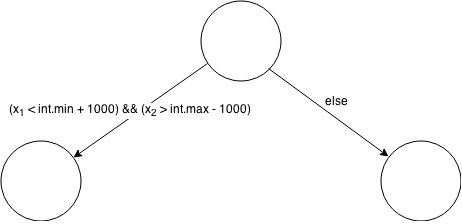
\includegraphics[width=0.7\linewidth]{ParameterTestCFG}
\caption{ParameterTestCFG}
\label{fig:ParameterTestCFG}
\end{figure}

The disease that ails the algorithm is most likely over designing to specific tests. This lead to some fundamental flaws in the handling of ranges and local optimization. The initial range search uses a single range for all parameters in a test case; if having all parameters in the same range fails to cover anything new then the range is declared not useful. This means if some coverage requires parameters from separate ranges, and these ranges are only useful when combined, the algorithm will perform on par with random search in its attempts to get that coverage. The LocalOptFromZero algorithm also fails miserably if coverage does not require parameters in the neighborhood of zero. When both these techniques were implemented coverage increased, and they were both tweaked to increase coverage even more; this gave the false impression the algorithm was getting better, but increasing coverage on the small number of CFGs at our disposal is not the same thing as increases quality of the algorithm.




\newpage
\section{Conclusion}


\subsection{Future Work}

\newpage
\section*{Appendix A}

The algorithm takes three input parameters, population size, mutation probability, and number of cut points. In order to find a good set of parameter, tests were run in which we kept just one variable constant while trying to optimize the other two. For example, a test would keep population size constant at 10 while letting the mutation probability range from 0.00 to 1.00 and letting the number of cut points range from 1 to 4. A ``step size'' is used to avoid trying too many values. We first test the mutation probability at 0.00 and then for the next test we step it up to its next value. Each parameter, with its starting value, ending value, and step size can be seen in the following table.

\begin{table}[h]
\begin{tabular}{l|l|l|l|l}
	\cline{2-4}
	                                 & Start & End & Step &  \\ \cline{1-4}
	\multicolumn{1}{|l|}{Population} & 5     & 100 & 5    &  \\ \cline{1-4}
	\multicolumn{1}{|l|}{Mutation}   & 0     & 1   & 0.05 &  \\ \cline{1-4}
	\multicolumn{1}{|l|}{Cut Points} & 1     & 4   & 1    &  \\ \cline{1-4}
\end{tabular}
\end{table}


\newpage
\begin{thebibliography}{9}

\bibitem{FraserTestSuites}
   Gordon Fraser, Andrea Arcuri,
   \emph{Whole Test Suite Generation}
   IEEE.
   2011.

\bibitem{Fraser}
   Gordon Fraser, Matt Statts, Phil McMinn, Andrea Arcuri, Frank Padberg\\
   \emph{Does Automated Unit Test Generation Really Help Software Testers? A Controlled Empirical Study}.
   ACM Transactions on Software Engineering and Methodology (TOSEM).
   2014
   
\bibitem{meyers1}
  G. Meyers,
  \emph{The Arts of Software Testing}.
  Hoboken, New Jersey: John Wiley \& Sons Inc.
  2nd edition,
   2004.
\bibitem{model2}
  M. Utting and B. Legeard,
  \emph{Practical Model-Based Testing: A Tools Approach}.
  San Francisco: Morgan-Kaufmann.
   2007.
\bibitem{chang3}
  	K.-H. Chang, J. H. C. II, W. H. Carlisle and D. B. Brown
  \emph{A framework for intelligent test data generation}.
  Journal of Intelligent and Robotic Systems
  vol. 5, 
  no. 2, 
  pp. 147-165, 
  April 1992.
\bibitem{sthammer4}
  	J. Wegener, H. Sthammer, B. Jones and D. Eyres,
  \emph{Testing real-time systems using genetic algorithms}.
  Software Quality Journal.
  pp. 127-135, 
  1997.    
\bibitem{apps5}
  X. S, E. C, S. C, L. G. A, K. S and K. K,
  \emph{Applications of Genetic Algorithms to Software Testing}.
  in Internation Conference on Software Engineering and its Applications, 
  Toulouse, 
  1992.\textbf{TODO: fix this citation}
  
\bibitem{limits6}
  	S. Aljahdali, Taif, A. Ghiduk and M. El-Telbany,
  \emph{The limitations of genetic algorithms in software testing}.
  in Computer Systems and Applications, 
  Hammamet, 
  2010. 
\bibitem{sthammer7}
  	B. F. Jones, H. H. Sthammer and D. Eyres,
  \emph{Automatic structural testing using genetic algorithms}.
  Software Engineering Journal, 
  pp. 299-306, 
  September 1996.  
\bibitem{pargas8}
  	R. P. Pargas, M. J. Harrold and R. R. Peck,
  \emph{Test-Data Generation Using Genetic Algorithms}.
  Journal of Software Testing, Verifcation, and Reliability, 
  1999.      
\end{thebibliography}

\end{document}